\chapter{The OpenStack Dashboard}
After login, you can see the Overview tab of \gls{Horizon}, the \gls{OpenStack Dashboard}.

\begin{center}
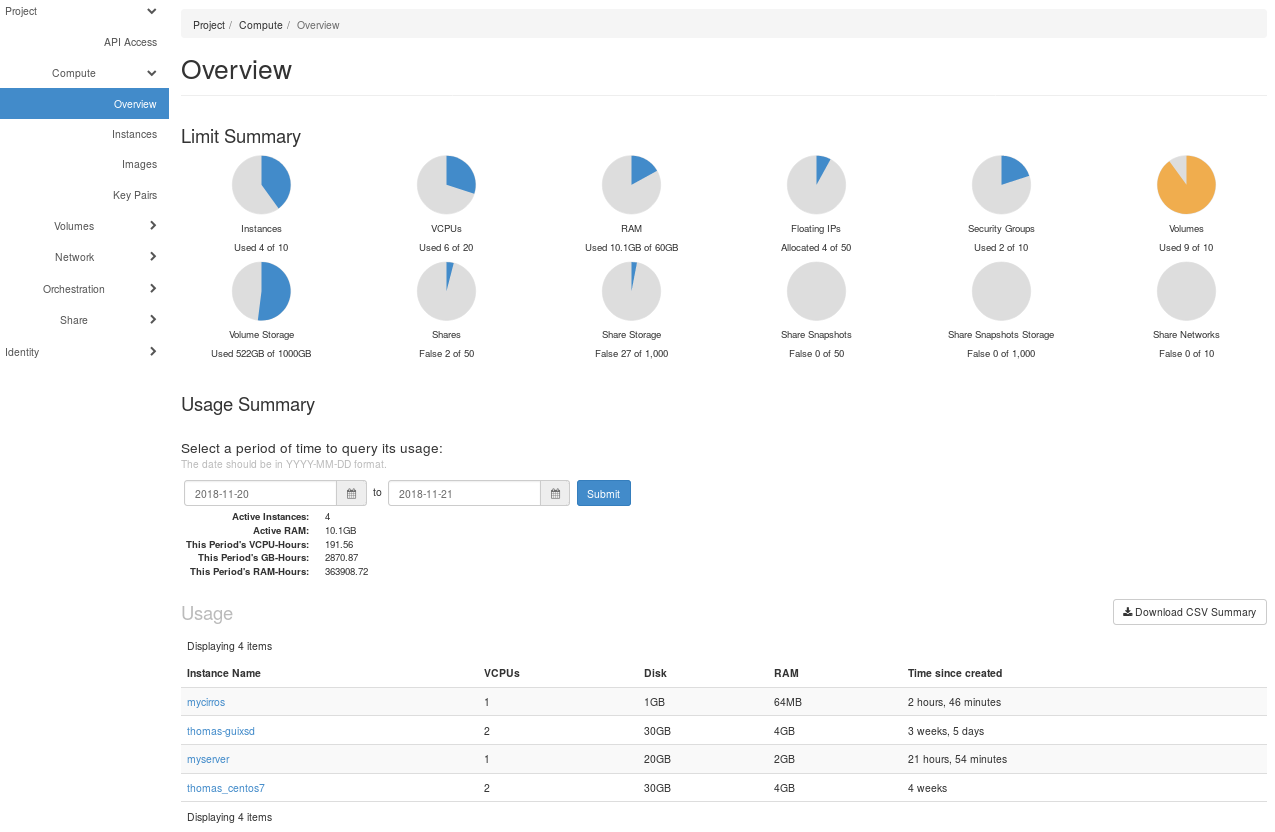
\includegraphics[width=\textwidth]{img/tab-compute-overview.png}
\end{center}

This chapter briefly describes the different components of the
dashboard.  You can read the official documentation at
\url{https://docs.openstack.org/horizon/\osversion/user}.

\strong{Note:} The VSC cloud uses a customized dashboard.  Some
features mentioned in the official OpenStack documentation were
intentionally removed, please contact \cloudinfo if you need access
to one of these disabled features.

\section*{Project tab}\label{sec:project-tab}
Resources (instances, data volumes, networks, \ldots) in OpenStack are
organized into different projects, and every user is a member of one
or more projects.  Every project member has full access to all of the
project's resources.

From the Project tab, you can access the following categories:
\begin{description}
\item[API Access] View API endpoints.
\item[Compute]\ 
\begin{itemize}
\item
  Overview: View reports for the project.
\item
  Instances: View, launch, create a snapshot from, stop, pause, or
  reboot instances, or connect to them through VNC.
\item
  Images: View images and instance snapshots created by project users,
  plus any images that are publicly available. Create, edit, and delete
  images, and launch instances from images and snapshots.
\item
  Key Pairs: View, create, edit, import, and delete key pairs.
\item
  Server Groups: Server groups provide a mechanism to group servers according to certain policy.
\end{itemize}
\item[Volumes]\ 
\begin{itemize}
\item
  Volumes: View, create, edit, and delete volumes.
\item
  Snapshots: View, create, edit, and delete volume snapshots.
\end{itemize}
\item[Network]\ 
\begin{itemize}
\item
  Networks: Create and manage public and private networks.
\item
  Security Groups: View, create, edit, and delete security groups and
  security group rules..
\item
  Floating IPs: Allocate an IP address to or release it from a project
\end{itemize}
\item[Orchestration]\ 
  \begin{itemize}
\item
  Stacks: Use the REST API to orchestrate multiple composite cloud applications.
\item
  Resource types: Show a list of all the supported resource types for HOT templates.
\item
  Template versions: The version of a Heat template specifies the format of the template and also the corresponding features that will be validated and supported.
\item
  Template generator: A graphical interface to build and edit templates.
\end{itemize}
\item[Shares]\ 
\begin{itemize}
\item Shares: Create and manage \gls{share}s.
\end{itemize}
\end{description}

\section*{Identity tab}\label{sec:identity-tab}
From the Identity tab, you can access the following categories:

\begin{description}
\item[Projects] View, create, assign users to, remove users from, and delete
  projects.
\item[Users] View, create, enable, disable, and delete users.
\item[Application Credentials] With application credentials, a user
  can grant applications limited access to their cloud resources.
\end{description}

%%% Local Variables:
%%% mode: latex
%%% TeX-master: "intro-Cloud"
%%% End:
